%%%%%%%%%%%%%%%%%%%%%%%%%%%%%%%%%%%%%%%%%
% baposter Landscape Poster
% LaTeX Template
% Version 1.0 (11/06/13)
%
% baposter Class Created by:
% Brian Amberg (baposter@brian-amberg.de)
%
% This template has been downloaded from:
% http://www.LaTeXTemplates.com
%
% License:
% CC BY-NC-SA 3.0 (http://creativecommons.org/licenses/by-nc-sa/3.0/)
%
%%%%%%%%%%%%%%%%%%%%%%%%%%%%%%%%%%%%%%%%%

%----------------------------------------------------------------------------------------
%	PACKAGES AND OTHER DOCUMENT CONFIGURATIONS
%----------------------------------------------------------------------------------------

\documentclass[portrait,letterpaper,fontscale=1]{xebaposter} % Adjust the font scale/size here

\usepackage{graphicx} % Required for including images
\graphicspath{{figures/}} % Directory in which figures are stored

\usepackage{amsmath} % For typesetting math
\usepackage{amssymb} % Adds new symbols to be used in math mode

\usepackage{booktabs} % Top and bottom rules for tables
\usepackage{enumitem} % Used to reduce itemize/enumerate spacing
\usepackage{palatino} % Use the Palatino font
\usepackage[font=small,labelfont=bf]{caption} % Required for specifying captions to tables and figures

\usepackage{multicol} % Required for multiple columns
\setlength{\columnsep}{1.5em} % Slightly increase the space between columns
\setlength{\columnseprule}{0mm} % No horizontal rule between columns

\usepackage{tikz} % Required for flow chart
\usetikzlibrary{shapes,arrows} % Tikz libraries required for the flow chart in the template

\newcommand{\compresslist}{ % Define a command to reduce spacing within itemize/enumerate environments, this is used right after \begin{itemize} or \begin{enumerate}
\setlength{\itemsep}{1pt}
\setlength{\parskip}{0pt}
\setlength{\parsep}{0pt}
}

\definecolor{lightblue}{rgb}{0.145,0.6666,1} % Defines the color used for content box headers

\addtolength{\topmargin}{-.25in}

\begin{document}

\begin{poster}
{
headerborder=closed, % Adds a border around the header of content boxes
colspacing=1em, % Column spacing
bgColorOne=white, % Background color for the gradient on the left side of the poster
bgColorTwo=white, % Background color for the gradient on the right side of the poster
borderColor=lightblue, % Border color
headerColorOne=black, % Background color for the header in the content boxes (left side)
headerColorTwo=lightblue, % Background color for the header in the content boxes (right side)
headerFontColor=white, % Text color for the header text in the content boxes
boxColorOne=white, % Background color of the content boxes
textborder=roundedleft, % Format of the border around content boxes, can be: none, bars, coils, triangles, rectangle, rounded, roundedsmall, roundedright or faded
eyecatcher=true, % Set to false for ignoring the left logo in the title and move the title left
headerheight=0.1\textheight, % Height of the header
headershape=roundedright, % Specify the rounded corner in the content box headers, can be: rectangle, small-rounded, roundedright, roundedleft or rounded
headerfont=\Large\bf\textsc, % Large, bold and sans serif font in the headers of content boxes
%textfont={\setlength{\parindent}{1.5em}}, % Uncomment for paragraph indentation
linewidth=2pt % Width of the border lines around content boxes
}
%----------------------------------------------------------------------------------------
%	TITLE SECTION 
%----------------------------------------------------------------------------------------
%
{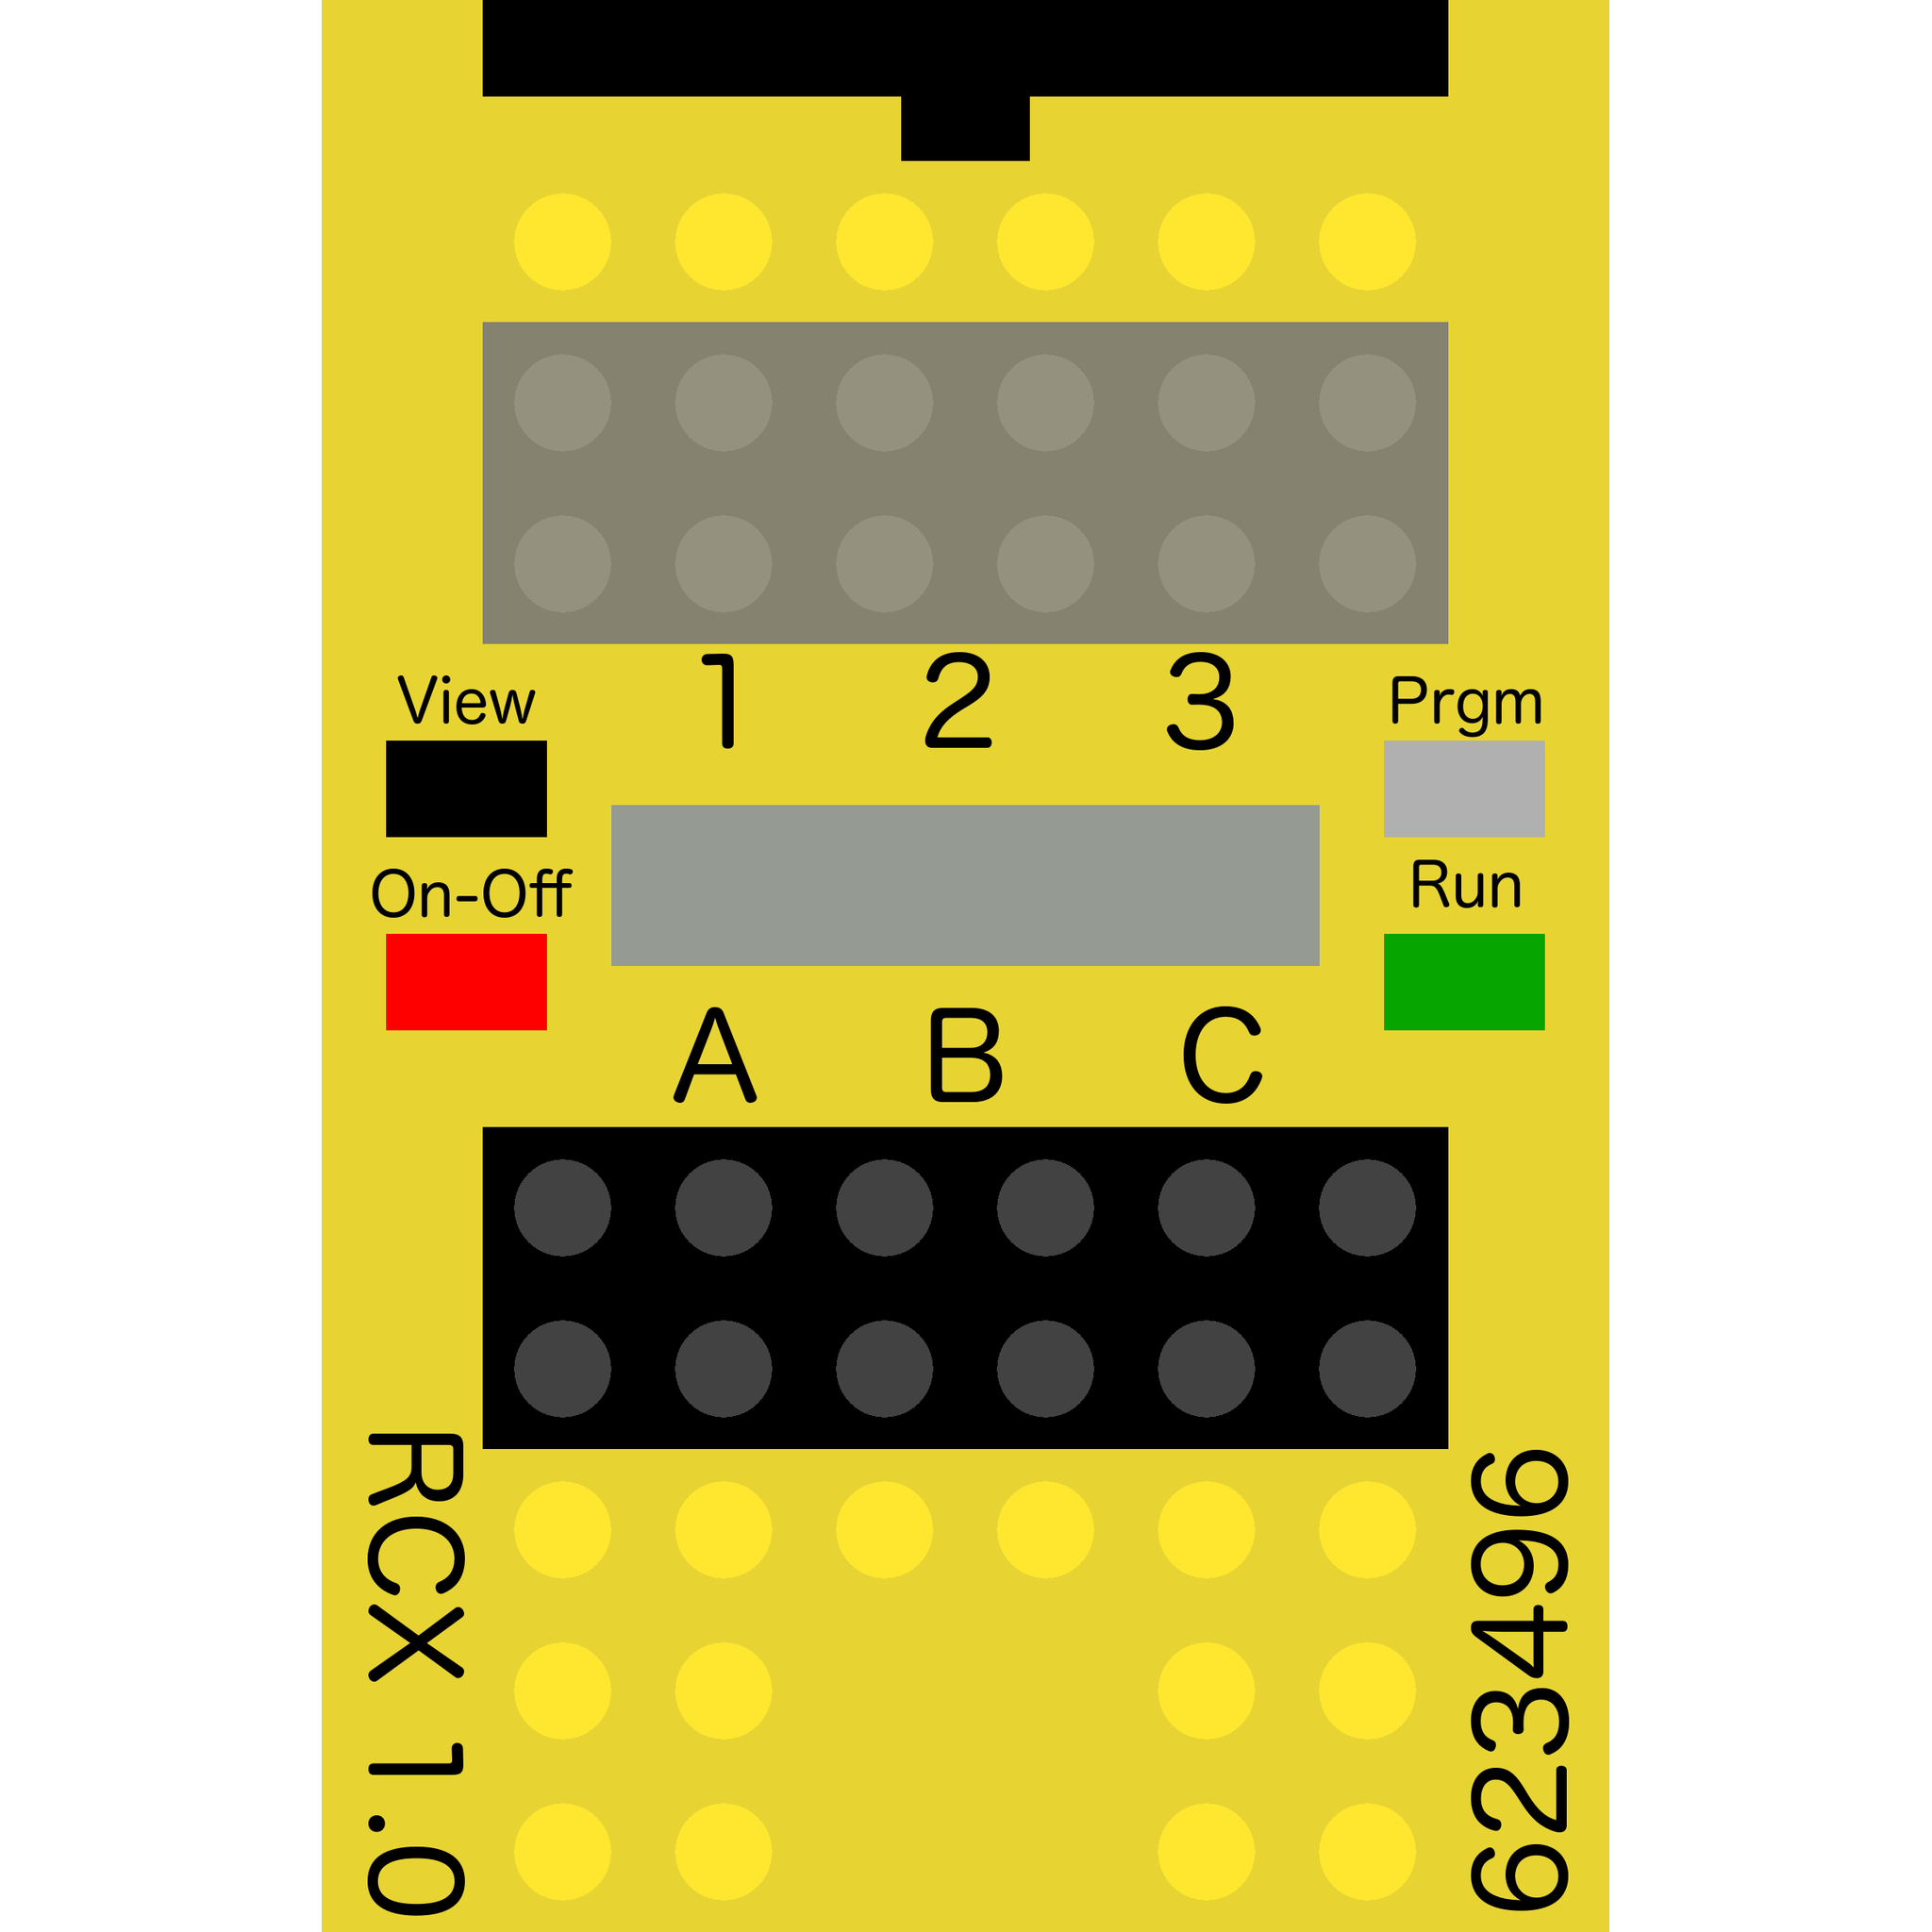
\includegraphics[height=5em]{rcx.png}} % First university/lab logo on the left
{\bf\textsc{About FaRCX}\vspace{0.5em}} % Poster title
{\textsc{John Holbrook, Philip Taylor}} % Author names and institution
{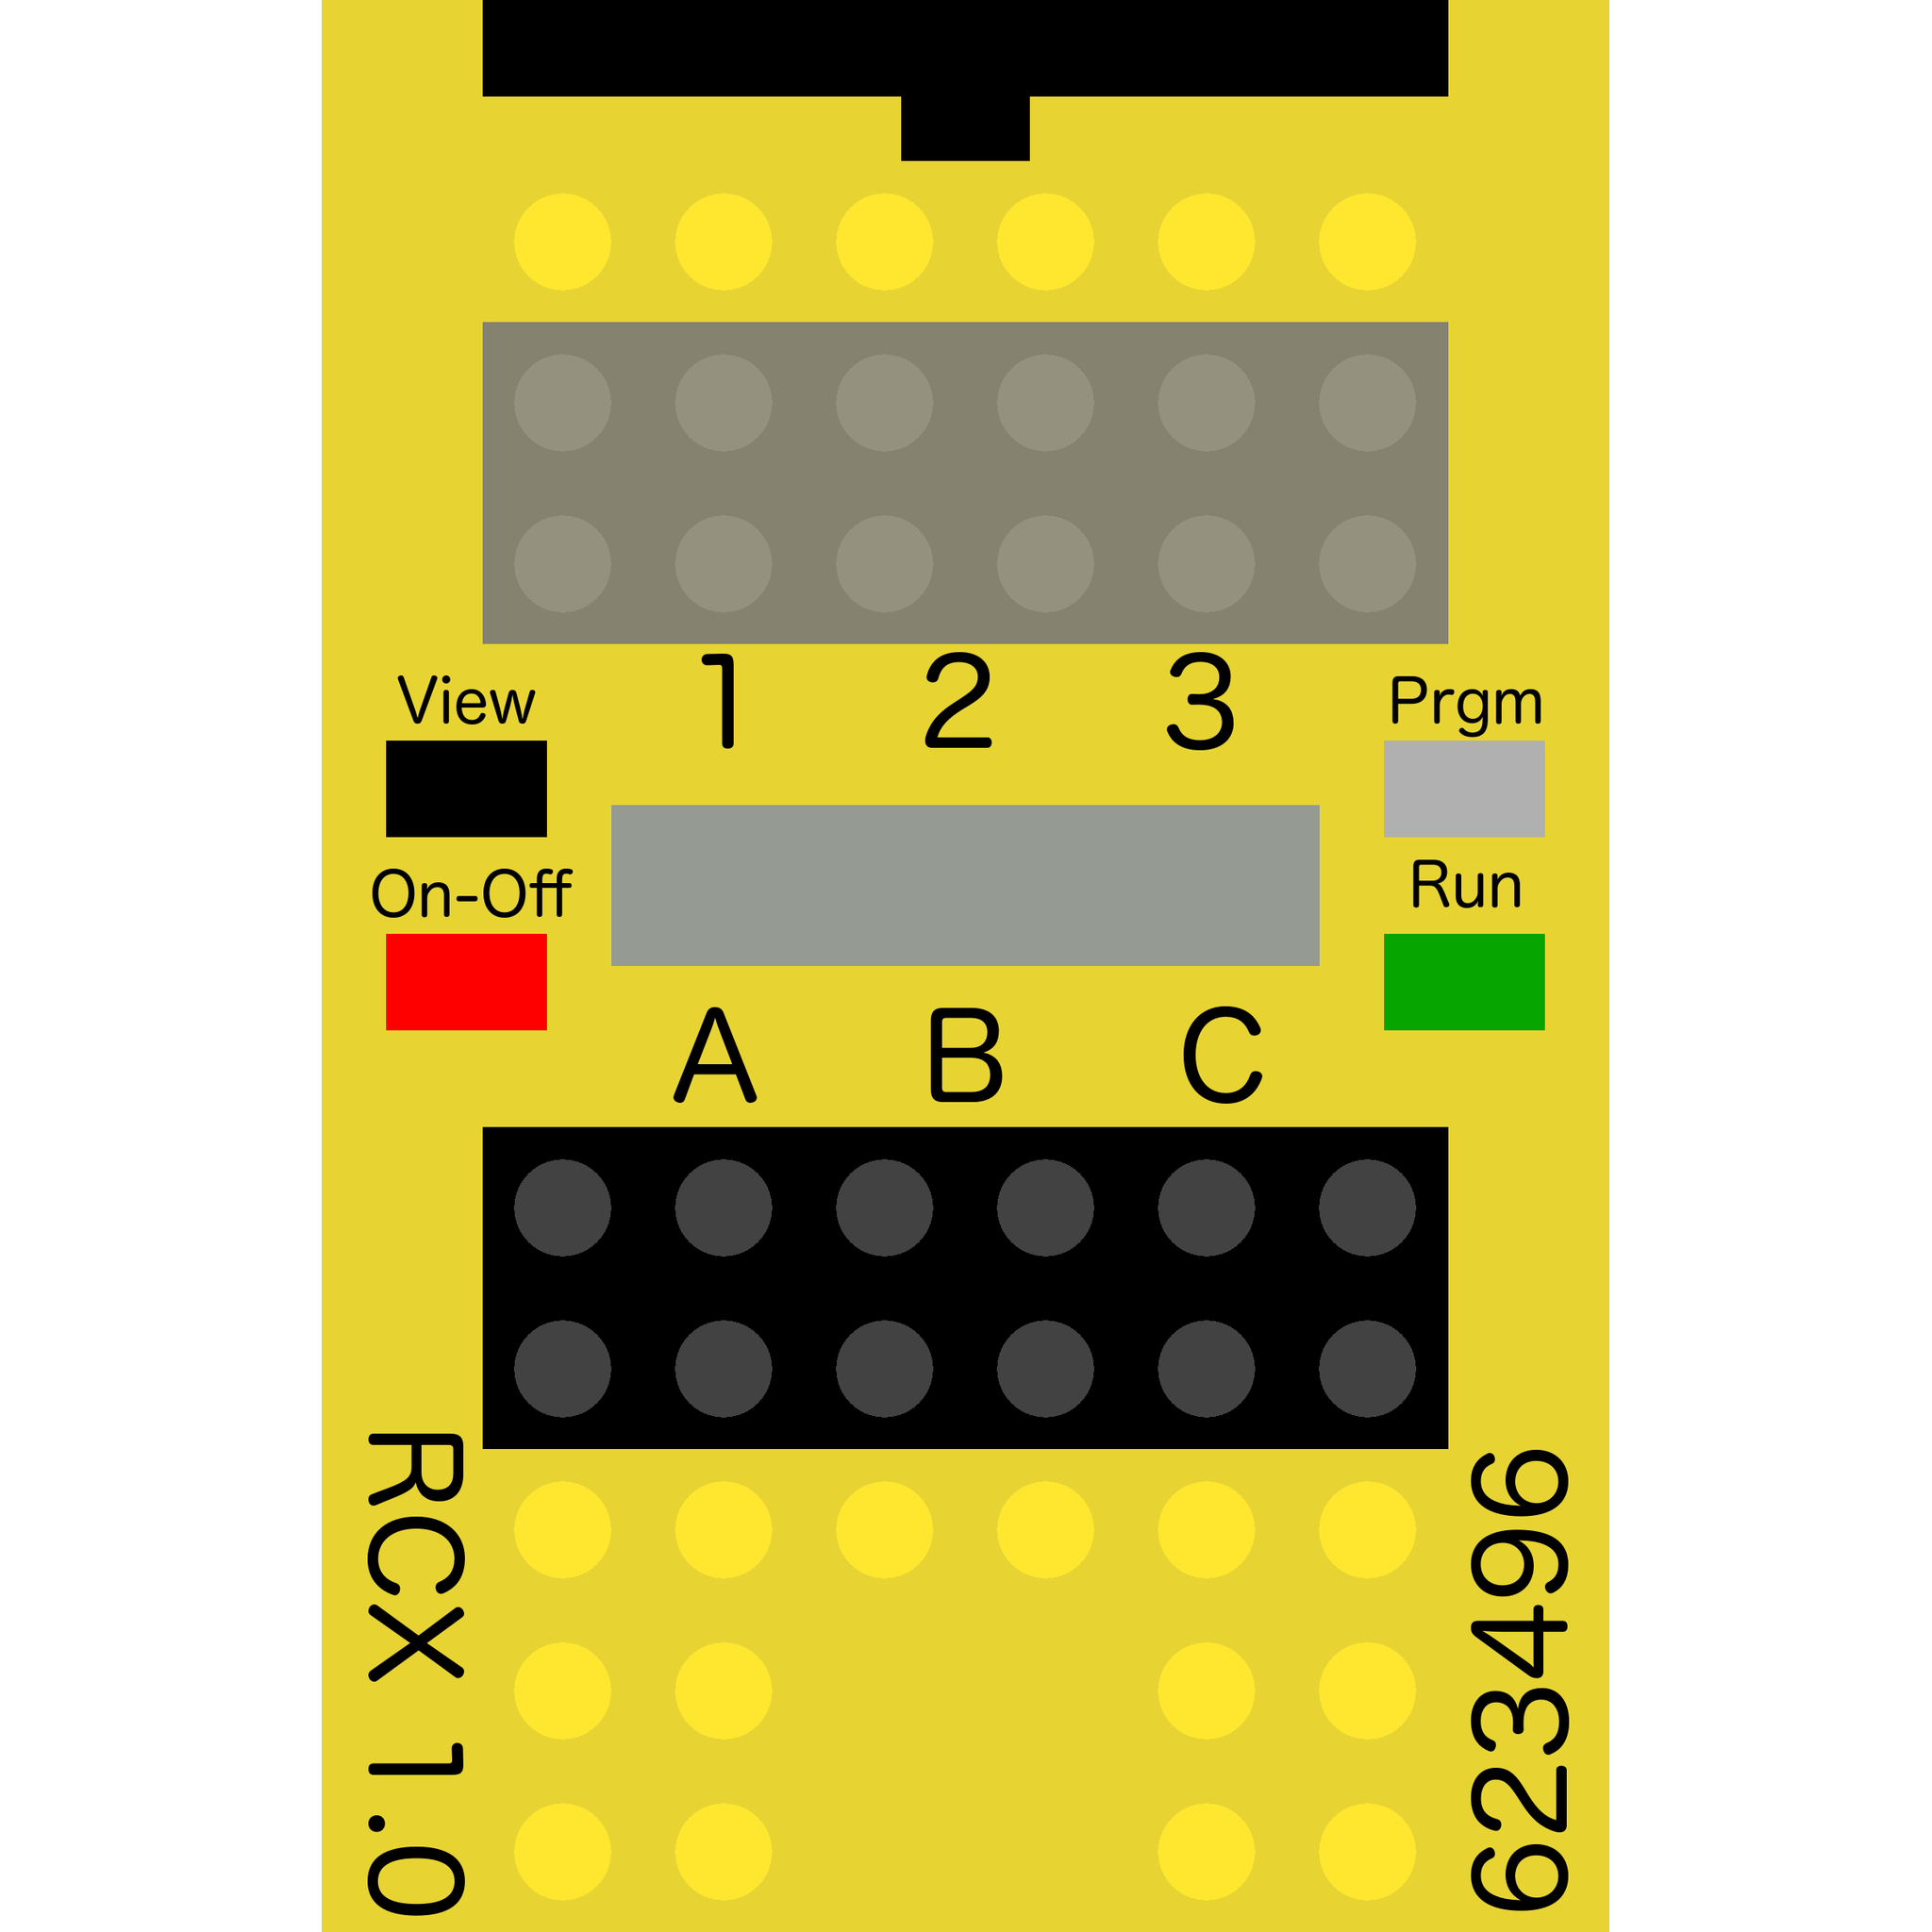
\includegraphics[height=5em]{rcx.png}} % Second university/lab logo on the right




%-----
\headerbox{Overview}{name=overview, span=3}{
	FaRCX is software for controllowing a LEGO\textregistered RCX robot over
	the internet with one or more live video feeds. The software is open-source
	and runs on modern Linux systems. The project is a spiritual successor to
	\textit{Red Rover, Red Rover}, a late-1990s project of LEGO and The
	Planetary Society. A permanent "Mars Rover" (actually located in
	Huntington, WV) can be driven online at http://farcx.com.
}


\headerbox{Previous Software}{name=prior-art, span=3, below=overview}{
	A previous software package, \textit{Red Rover, Red Rover}, also allowed for
	teleoperation, but had several limitations:
	\begin{itemize}\compresslist
		\item \textit{RRRR}, developed in 1998 for The Planetary Society, had long since been
		abandoned as a coordinated project.
		\item Server software was Windows-only, and unsupported on recent versions of Windows.
		\item Video was limited to a single camera, and limited to still images transmitted during
		control sequences (otherwise static).
		\item Control web page design was clunky and difficult to navigate.
	\end{itemize}
	In the early 2000s, as many as one dozen \textit{RRRR} deployments,
	located around the world, were available online. FaRCX was designed to
	replace the last known \textit{RRRR} deployment, originally maintained
	by Linda Hamilton of Marshall University. The FaRCX software took control of the rover model in January 2015.
}

\headerbox{Advantages of FaRCX}{name=advantages, span=3, below=prior-art}{
	\begin{itemize}\compresslist
		\item Project is open-source, with continued support.
		\item Software stack designed to run on Linux, but could be reatively easily adapted to run on other platforms.
		\item Video is live-streamed at variable frame rate (4 FPS used for remote rover), and
			multiple cameras can be utilized (onboard, third-person view, etc.)
		\item Control web page written to comply with modern HTML standards.
		\item Control of robot is achieved by sending easily-decipherable POST requests to a
			server, so other means of control (scripts, smartphone apps, etc.)
			could easily be developed.
	\end{itemize}
}

\headerbox{Photos}{name=photos, span=3, below=advantages}{
	\begin{multicols}{2}
		\begin{center}
			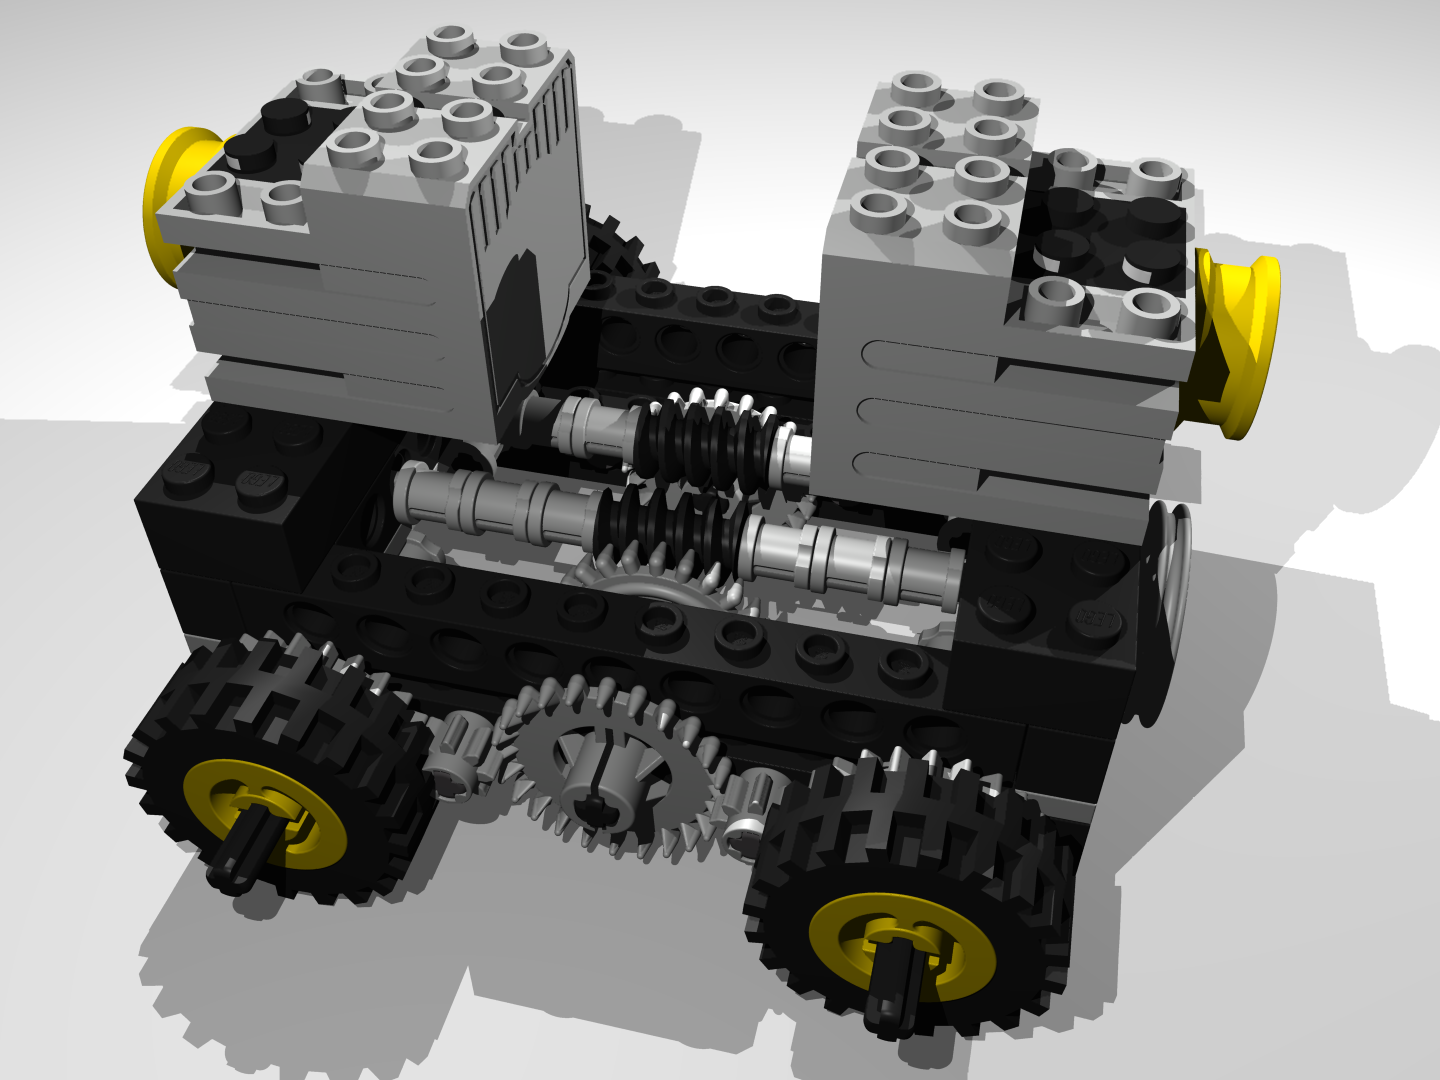
\includegraphics[width=0.95\linewidth]{rover.png}\\
			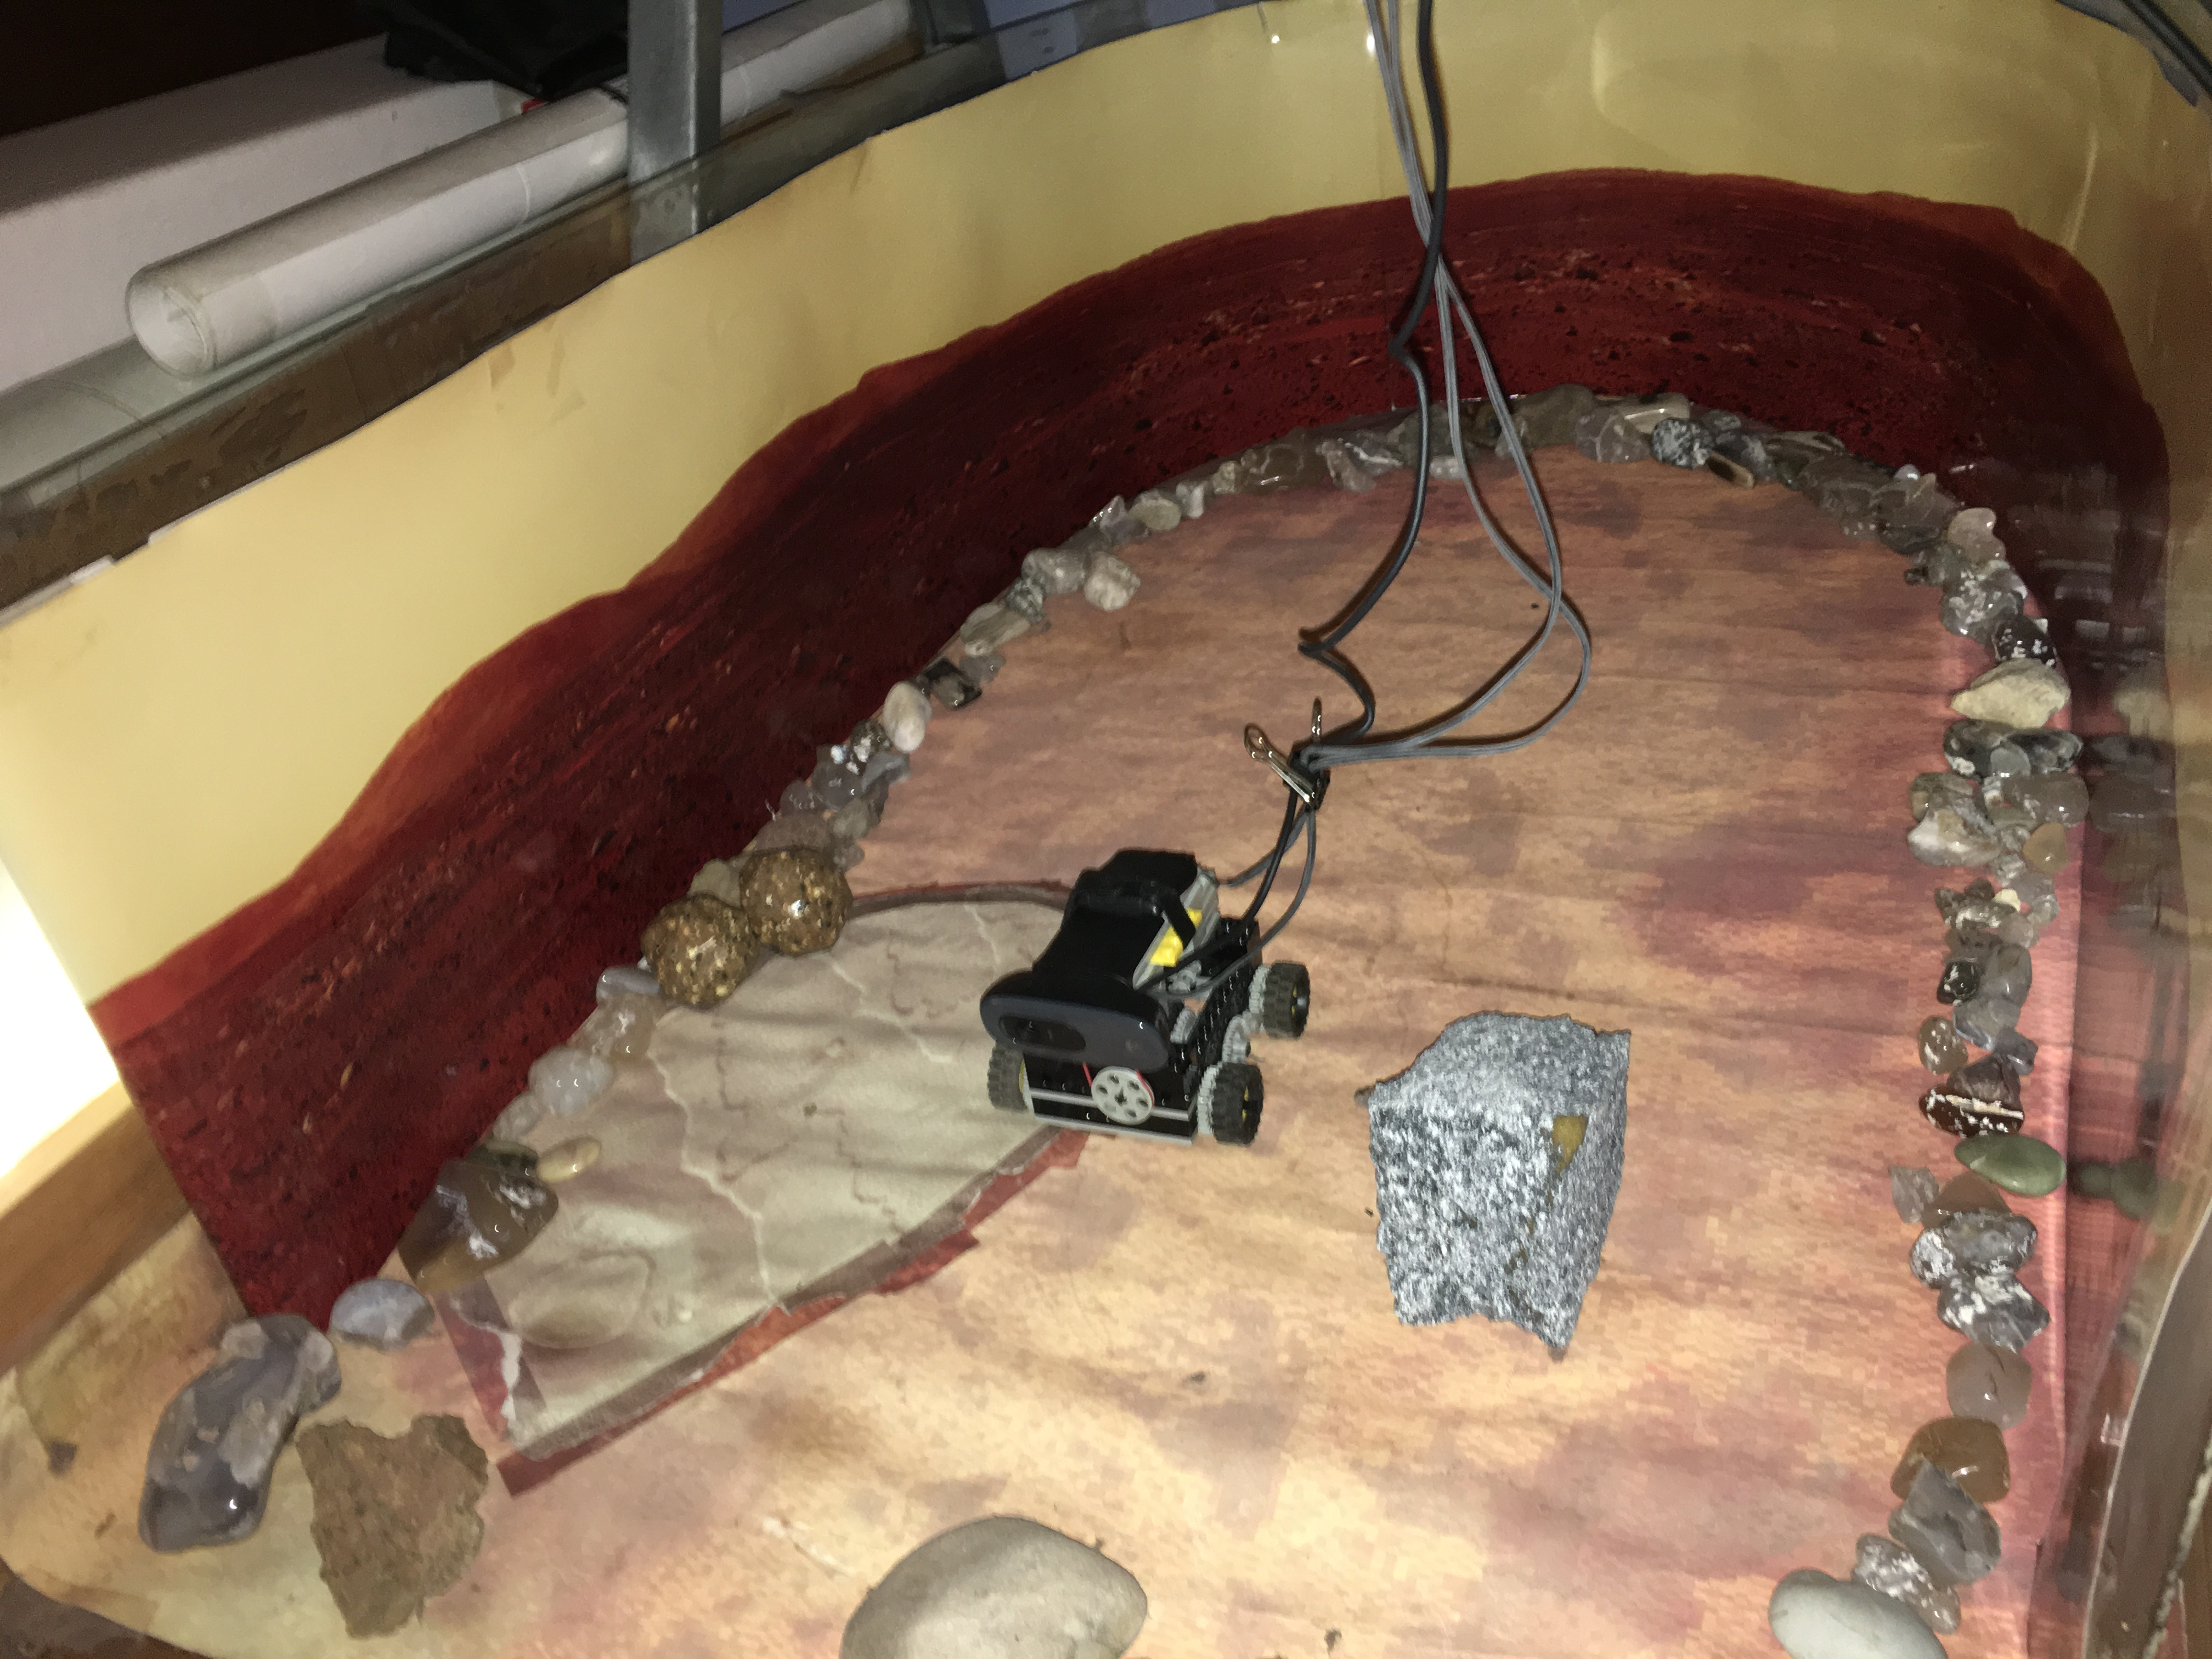
\includegraphics[width=0.95\linewidth]{mars_diorama.jpg}\\			
		\end{center}
	\end{multicols}
}


\headerbox{}{name=filler-bar, span=3, below=photos}{
	\begin{center}
		\huge{DRIVE OUR ROVER AT HTTP://FARCX.COM!}
	\end{center}
}

%-----
\end{poster}

\end{document}